\documentclass[11pt]{beamer}
% Packages
\usepackage{beamer-german}

% Title etc.
\title{Politische Unterstützung}
\subtitle{Analyse politischer Unterstützung in der quantitativen Forschungspraxis}
\date{29. Oktober 2021}
\author{B. Philipp Kleer}
\institute{Institut für Politikwissenschaft | Justus-Liebig-Universität Gießen}

\setbeamerfont{itemize/enumerate body}{size = \small}
\setbeamerfont{itemize/enumerate subbody}{size = \footnotesize}
\setbeamerfont{itemize/enumerate subsubbody}{size = \scriptsize}

% Datumspaket
\usepackage[german]{isodate}

% Table packages
\usepackage{booktabs}
\usepackage{longtable}

% bibtex-file
\addbibresource{lit-s2.bib} 

\begin{document}

\begin{frame}
	\maketitle
\end{frame}

\begin{frame}[t]{Heutige Agenda}
\shine{Grundlagentexte}
	\begin{itemize}
		\item \fullcite{Easton1975}
		\item \fullcite{Fuhse2005}  (S. 20-63)
		\pause
		\item[$\Rightarrow$] Verständnisprobleme / Klärungsfragen?
		\item[$\Rightarrow$] Wie wirken direkten Erfahrungen bei \textit{specific support} und \textit{diffuse support}?
		\item[$\Rightarrow$] Zeit: 20 Minuten (kommen Sie zurück ins Plenum, wenn Sie schon vor der Zeit durch sind)
	\end{itemize}
\end{frame}

\begin{frame}[t]{4 Bilder \& Eastons Theorie}
So, wir haben jetzt Grundfragen geklärt. Dieses Wissen vertiefen wir nun angewandt. Jede Gruppe bekommt eins der vier Bilder zugeteilt und soll frei assoziieren mit Eastons Theorie. \\
\shine{Zeit}: 15 Minuten; Präsentation in Plenum: 5 Minuten
	\begin{columns}
		\begin{column}{0.25\textwidth}
			\begin{figure}[ht]
				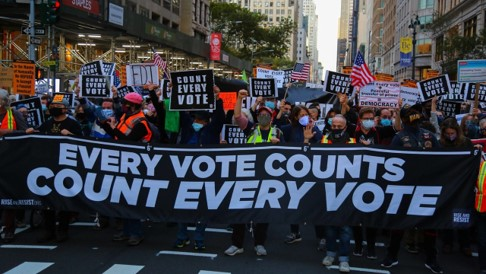
\includegraphics[width=\textwidth]{pics/s2-1.jpg}
			\end{figure}
		\end{column}
		\begin{column}{0.25\textwidth}
			\begin{figure}[ht]
				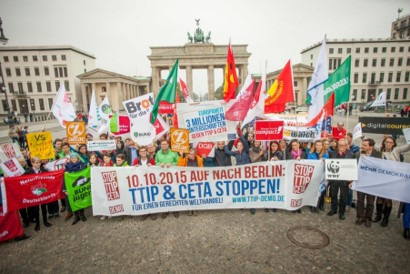
\includegraphics[width=\textwidth]{pics/s2-2.jpg}
			\end{figure}
		\end{column}
		\begin{column}{0.25\textwidth}
			\begin{figure}[ht]
				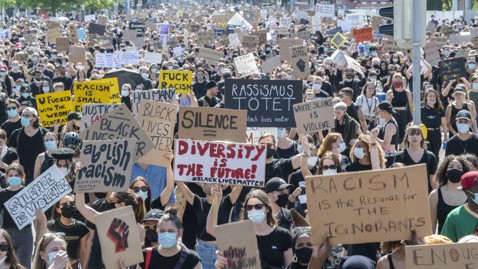
\includegraphics[width=\textwidth]{pics/s2-3.jpg}
			\end{figure}
		\end{column}
		\begin{column}{0.25\textwidth}
			\begin{figure}[ht]
				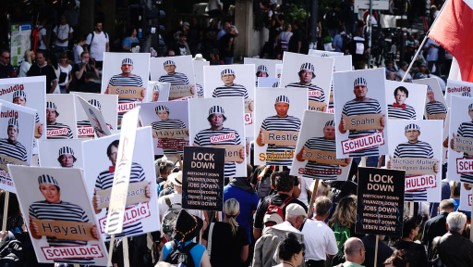
\includegraphics[width=\textwidth]{pics/s2-4.jpg}
			\end{figure}
		\end{column}
	\end{columns}
\end{frame}

\begin{frame}{Werte, Einstellungen \& Handeln}
	\begin{center}
		\begin{figure}[ht]
			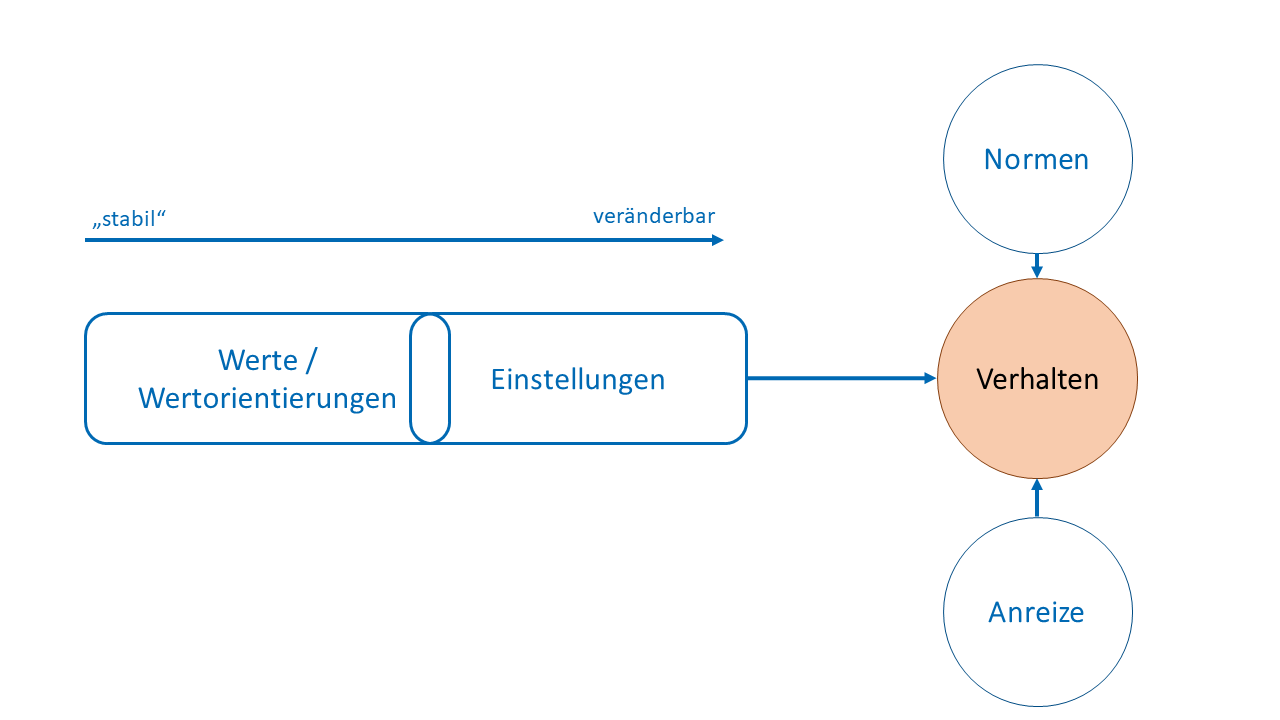
\includegraphics[width=\textwidth]{pics/s2-5.png}
		\end{figure}
	\end{center}
\end{frame}

\begin{frame}{Wertemodell nach \cite{Schwartz1992}}
	\begin{columns}
		\begin{column}{0.5\textwidth}
			\begin{figure}[ht]
				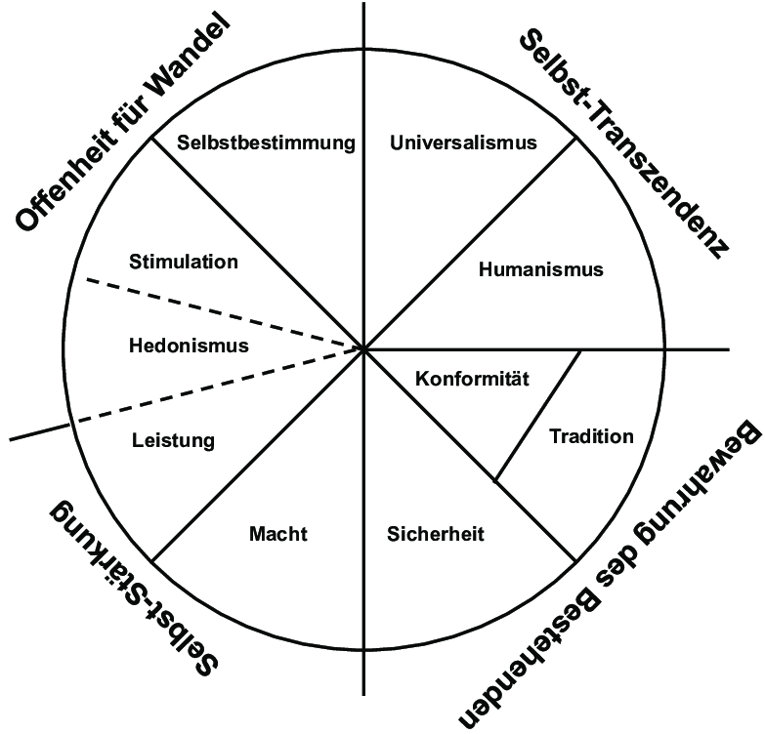
\includegraphics[width=\textwidth]{pics/s2-6.png}
			\end{figure}
		\end{column}
		\begin{column}{0.5\textwidth}
			„ [...] conceptions of the desirable that guide the way social actors (e.g. organisational leaders, policy-makers, individual persons) select actions, evaluate people and events, and explain their actions and evaluations” \parencite[24f]{Schwartz1992}.
		\end{column}
	\end{columns}
\end{frame}

\begin{frame}[t]{Politisches System}
\shine{Definition:} \\ \pause
Interaktionen innerhalb einer Gesellschaft, die mit der autoritativen Allokation von Werten beschäftigt sind \parencite[129ff]{Easton1965}\\  \pause
\shine{Was sind Werte hier?} \\ \pause
materielle und ideelle Güter

\end{frame}

\begin{frame}[t]{Modell des Politischen System}
Kann jemand das Modell grob skizzieren? \\

	\begin{figure}[ht]
		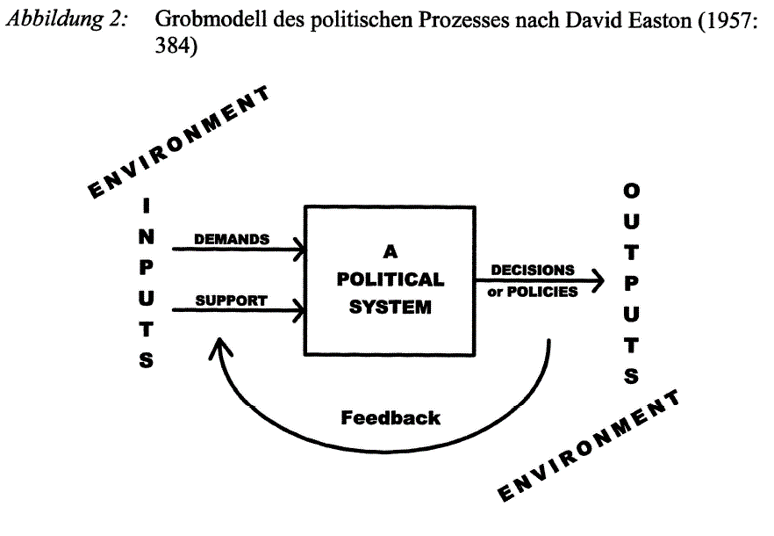
\includegraphics[width=\textwidth]{pics/s2-7.png}
	\end{figure}
\end{frame}

\begin{frame}[t]{Politische Unterstützung}
Welche zwei Formen werden unterschieden? \\ \pause

\begin{itemize}
	\item diffuse
	\item specific \pause
\end{itemize}

Wohin richtet sich politische Unterstützung? \pause
\begin{itemize}
	\item political community
	\item regime
	\item authorities
\end{itemize}
\end{frame}

\begin{frame}[t]{Objekte politischer Unterstützung}
\shine{Entscheidungsträger:innen (authorities)} \\ \pause

„They must engage in the \shine{daily affairs} of a political system; they must be \shine{recognized by most members} of the system as \shine{having the responsibility for these matters}; and \shine{their actions must be accepted as binding} most of the time by most of the member \shine{as long as they act within the limits of their roles}“ \parencite[212]{Easton1965} \\ \pause

z.B.: Kanzler:in, Fraktionsführer:in, Partei-Vorsitzende:r, Minister:in etc. 
\end{frame}

\begin{frame}[t]{Objekte politischer Unterstützung}
\shine{Regime} \\ \pause

„The regime as \shine{sets of constraints on political interaction} in all systems may be broken down into three components: \shine{values} (goals and principles), \shine{norms}, and \shine{structure of authority}.“ \parencite[193]{Easton1965}\\ \pause

\textit{Values}: Ideologien (Demokratie, Kommunismus, Nationalsozialismus) \\ \pause

\textit{Norms}: Spielregeln des jeweiligen Systems, wie laufen Prozesse ab \\ \pause

\textit{Authority structure}: Befugnisse einzelner politischer Ämter \\ \pause
\end{frame}

\begin{frame}[t]{Objekte politischer Unterstützung}
\shine{Politische Gemeinschaft (political community)} \\ \pause

„In confining the idea of political community in this way, I do so in order to focus (…) on the group of members who are drawn together by the fact that \shine{they participate in a common structure and a set of processes}, however tight or loose the ties may be.“ \parencite[178]{Easton1965} \\ \pause

z.B.: „Wir-Gefühl“, Nationalstolz, Verbundenheitsgefühl 

\end{frame}

\begin{frame}{Entstehung politischer Unterstützung}
	\begin{figure}[ht]
		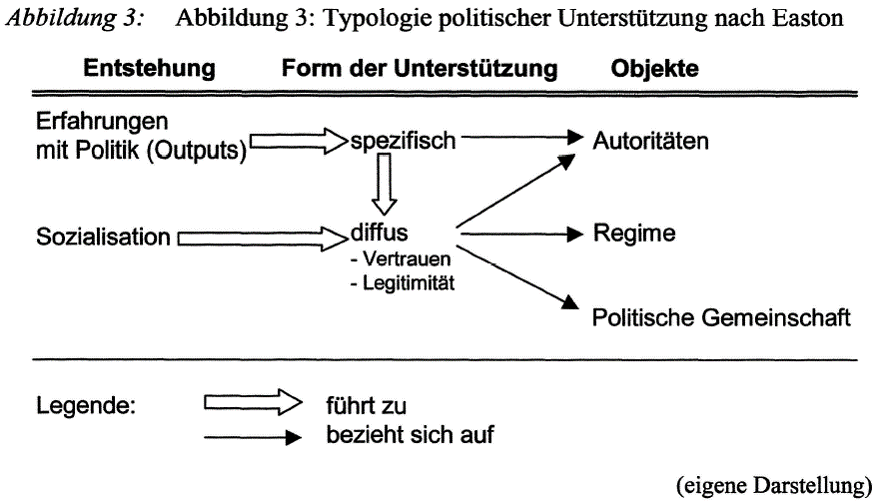
\includegraphics[width=\textwidth]{pics/s2-8.png}
		\caption{\cite[45]{Fuhse2005}}
	\end{figure}
\end{frame}

\begin{frame}[t]{Legitimität \& Vertrauen}
\shine{Legitimacy} \\ 
Worin besteht die Hauptverknüpfung? Welche Form? Auf welche Objekte? \\ \pause

\shine{Trust} \\
Worin unterscheidet sich \textit{trust} von \textit{legitimacy}? \\
\end{frame}

\begin{frame}[t]{Output \& Feedback}
\shine{Output} \\  \pause
\begin{itemize}
	\item kollektiv bindende Entscheidungen, die im politischen System getroffen wurden \pause
	\item Evaluierung durch Personen, davon abhängig neue Forderungen bzw. Unterstützung \pause
	\item[$\Rightarrow$] \textit{feedback loop}
\end{itemize}

\end{frame}

\begin{frame}[t]{Politische Unterstützung}
Was ist Kernmerkmal dieser Theorie? \\ \pause

	\begin{itemize}
		\item Politisches System ist black box \pause
		\item Es geht nicht darum Prozesse innerhalb des Politischen Systems zu erklären!
	\end{itemize}

\end{frame}

\begin{frame}{Rückfragen?}
	\begin{figure}[ht]
		
\includegraphics[width=0.25\textwidth]{pics/s2-9.png}
	\end{figure}

\end{frame}

\renewcommand*{\bibfont}{\scriptsize}

\begin{frame}[allowframebreaks]{Literatur}
	\nocite{*}
	\printbibliography[heading = none]
\end{frame}

\section{Wir sehen uns in zwei Wochen!}

\end{document}